\section*{Экспериментальная установка:}
    \begin{figure}[h!]
        \noindent\centering{
            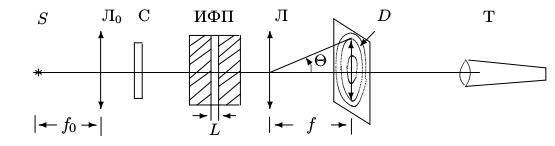
\includegraphics[height = 4cm]{020.png}
        }
        \caption{Схема экспериментальной установки}
    \end{figure} 
    Схема экспериментальной установки приведена на рис. 1. Свет от лампы S, пройдя через линзу Л 0 и светофильтр С, попадает на интерферометр Фабри—Перо (ИФП). Линза $L_0$ служит для формирования пучка лучей (слегка сходящегося или слегка расходящегося). Интерференционные кольца наблюдаются в фокальной плоскости линзы Л. Картина рассматривается через зрительную трубу Т, сфокусированную на эту плоскость. Диаметры колец измеряются с помощью микроскопа катетометра. Зрительная труба Т, отсчётный микроскоп — элементы катетометра — прибора, предназначенного для измерения расстояний в вертикальной плоскости вдоль вертикальной оси.